% Figure from MATH 591 notes, section 7. Compile with the notes preamble.
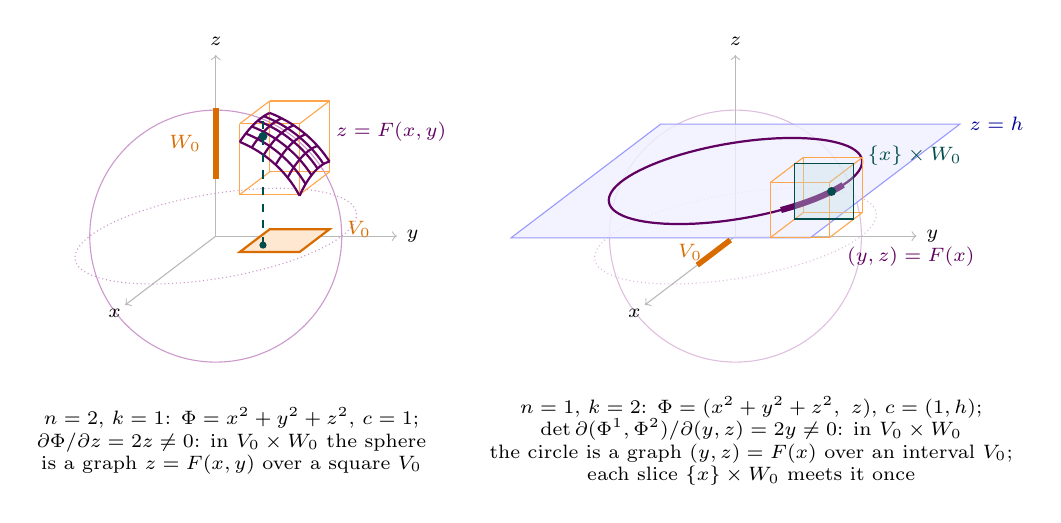
\begin{tikzpicture}[font=\scriptsize]
\begin{scope}[x={(-0.5cm,-0.38cm)}, y={(1cm,0cm)}, z={(0cm,1cm)}]
\draw[violet!40] (0,0,0) circle (1.6cm);
\draw[violet!40, densely dotted] plot coordinates {(1.6,0,0) (1.595,0.126,0) (1.58,0.25,0) (1.556,0.374,0) (1.522,0.494,0) (1.478,0.612,0) (1.426,0.726,0) (1.364,0.836,0) (1.294,0.94,0) (1.217,1.039,0) (1.131,1.131,0) (1.039,1.217,0) (0.94,1.294,0) (0.836,1.364,0) (0.726,1.426,0) (0.612,1.478,0) (0.494,1.522,0) (0.374,1.556,0) (0.25,1.58,0) (0.126,1.595,0) (0,1.6,0) (-0.126,1.595,0) (-0.25,1.58,0) (-0.374,1.556,0) (-0.494,1.522,0) (-0.612,1.478,0) (-0.726,1.426,0) (-0.836,1.364,0) (-0.94,1.294,0) (-1.039,1.217,0) (-1.131,1.131,0) (-1.217,1.039,0) (-1.294,0.94,0) (-1.364,0.836,0) (-1.426,0.726,0) (-1.478,0.612,0) (-1.522,0.494,0) (-1.556,0.374,0) (-1.58,0.25,0) (-1.595,0.126,0) (-1.6,0,0) (-1.595,-0.126,0) (-1.58,-0.25,0) (-1.556,-0.374,0) (-1.522,-0.494,0) (-1.478,-0.612,0) (-1.426,-0.726,0) (-1.364,-0.836,0) (-1.294,-0.94,0) (-1.217,-1.039,0) (-1.131,-1.131,0) (-1.039,-1.217,0) (-0.94,-1.294,0) (-0.836,-1.364,0) (-0.726,-1.426,0) (-0.612,-1.478,0) (-0.494,-1.522,0) (-0.374,-1.556,0) (-0.25,-1.58,0) (-0.126,-1.595,0) (0,-1.6,0) (0.126,-1.595,0) (0.25,-1.58,0) (0.374,-1.556,0) (0.494,-1.522,0) (0.612,-1.478,0) (0.726,-1.426,0) (0.836,-1.364,0) (0.94,-1.294,0) (1.039,-1.217,0) (1.131,-1.131,0) (1.217,-1.039,0) (1.294,-0.94,0) (1.364,-0.836,0) (1.426,-0.726,0) (1.478,-0.612,0) (1.522,-0.494,0) (1.556,-0.374,0) (1.58,-0.25,0) (1.595,-0.126,0) (1.6,0,0)};
\draw[->, gray!55] (0,0,0) -- (2.3,0,0) node[below left=-2pt, text=black] {$x$};
\draw[->, gray!55] (0,0,0) -- (0,2.3,0) node[right, text=black] {$y$};
\draw[->, gray!55] (0,0,0) -- (0,0,2.3) node[above, text=black] {$z$};
\fill[orange!18] (-0.23,0.57,0) -- (0.53,0.57,0) -- (0.53,1.33,0) -- (-0.23,1.33,0) -- cycle;
\draw[orange!85!black, thick] (-0.23,0.57,0) -- (0.53,0.57,0) -- (0.53,1.33,0) -- (-0.23,1.33,0) -- cycle;
\node[orange!85!black, anchor=west] at (-0.23,1.43,0) {$V_0$};
\draw[orange!85!black, line width=2pt] (0,0,0.729) -- (0,0,1.629) node[midway, left=1pt] {$W_0$};
\draw[orange!70, thin] (-0.23,0.57,0.729) -- (-0.23,0.57,1.629);
\draw[orange!70, thin] (-0.23,0.57,0.729) -- (-0.23,1.33,0.729);
\draw[orange!70, thin] (-0.23,0.57,0.729) -- (0.53,0.57,0.729);
\draw[orange!70, thin] (-0.23,0.57,1.629) -- (-0.23,1.33,1.629);
\draw[orange!70, thin] (-0.23,0.57,1.629) -- (0.53,0.57,1.629);
\draw[orange!70, thin] (-0.23,1.33,0.729) -- (-0.23,1.33,1.629);
\draw[orange!70, thin] (-0.23,1.33,0.729) -- (0.53,1.33,0.729);
\draw[orange!70, thin] (-0.23,1.33,1.629) -- (0.53,1.33,1.629);
\draw[orange!70, thin] (0.53,0.57,0.729) -- (0.53,0.57,1.629);
\draw[orange!70, thin] (0.53,0.57,0.729) -- (0.53,1.33,0.729);
\draw[orange!70, thin] (0.53,0.57,1.629) -- (0.53,1.33,1.629);
\draw[orange!70, thin] (0.53,1.33,0.729) -- (0.53,1.33,1.629);
\draw[violet!75!black, thick] plot coordinates {(-0.23,0.57,1.477) (-0.23,0.608,1.462) (-0.23,0.646,1.446) (-0.23,0.684,1.428) (-0.23,0.722,1.409) (-0.23,0.76,1.389) (-0.23,0.798,1.368) (-0.23,0.836,1.345) (-0.23,0.874,1.32) (-0.23,0.912,1.294) (-0.23,0.95,1.267) (-0.23,0.988,1.237) (-0.23,1.026,1.206) (-0.23,1.064,1.173) (-0.23,1.102,1.137) (-0.23,1.14,1.099) (-0.23,1.178,1.058) (-0.23,1.216,1.014) (-0.23,1.254,0.967) (-0.23,1.292,0.915) (-0.23,1.33,0.859)};
\draw[violet!75!black, thick] plot coordinates {(-0.23,0.57,1.477) (-0.192,0.57,1.483) (-0.154,0.57,1.487) (-0.116,0.57,1.491) (-0.078,0.57,1.493) (-0.04,0.57,1.494) (-0.002,0.57,1.495) (0.036,0.57,1.495) (0.074,0.57,1.493) (0.112,0.57,1.491) (0.15,0.57,1.487) (0.188,0.57,1.483) (0.226,0.57,1.478) (0.264,0.57,1.472) (0.302,0.57,1.464) (0.34,0.57,1.456) (0.378,0.57,1.446) (0.416,0.57,1.436) (0.454,0.57,1.424) (0.492,0.57,1.412) (0.53,0.57,1.398)};
\draw[violet!75!black, thick] plot coordinates {(-0.078,0.57,1.493) (-0.078,0.608,1.478) (-0.078,0.646,1.462) (-0.078,0.684,1.444) (-0.078,0.722,1.426) (-0.078,0.76,1.406) (-0.078,0.798,1.385) (-0.078,0.836,1.362) (-0.078,0.874,1.338) (-0.078,0.912,1.312) (-0.078,0.95,1.285) (-0.078,0.988,1.256) (-0.078,1.026,1.225) (-0.078,1.064,1.192) (-0.078,1.102,1.157) (-0.078,1.14,1.12) (-0.078,1.178,1.08) (-0.078,1.216,1.037) (-0.078,1.254,0.991) (-0.078,1.292,0.941) (-0.078,1.33,0.886)};
\draw[violet!75!black, thick] plot coordinates {(-0.23,0.722,1.409) (-0.192,0.722,1.415) (-0.154,0.722,1.42) (-0.116,0.722,1.423) (-0.078,0.722,1.426) (-0.04,0.722,1.427) (-0.002,0.722,1.428) (0.036,0.722,1.427) (0.074,0.722,1.426) (0.112,0.722,1.423) (0.15,0.722,1.42) (0.188,0.722,1.415) (0.226,0.722,1.41) (0.264,0.722,1.403) (0.302,0.722,1.396) (0.34,0.722,1.387) (0.378,0.722,1.377) (0.416,0.722,1.366) (0.454,0.722,1.354) (0.492,0.722,1.34) (0.53,0.722,1.326)};
\draw[violet!75!black, thick] plot coordinates {(0.074,0.57,1.493) (0.074,0.608,1.478) (0.074,0.646,1.462) (0.074,0.684,1.445) (0.074,0.722,1.426) (0.074,0.76,1.406) (0.074,0.798,1.385) (0.074,0.836,1.362) (0.074,0.874,1.338) (0.074,0.912,1.313) (0.074,0.95,1.285) (0.074,0.988,1.256) (0.074,1.026,1.225) (0.074,1.064,1.193) (0.074,1.102,1.158) (0.074,1.14,1.12) (0.074,1.178,1.08) (0.074,1.216,1.037) (0.074,1.254,0.991) (0.074,1.292,0.941) (0.074,1.33,0.886)};
\draw[violet!75!black, thick] plot coordinates {(-0.23,0.874,1.32) (-0.192,0.874,1.326) (-0.154,0.874,1.331) (-0.116,0.874,1.335) (-0.078,0.874,1.338) (-0.04,0.874,1.34) (-0.002,0.874,1.34) (0.036,0.874,1.34) (0.074,0.874,1.338) (0.112,0.874,1.336) (0.15,0.874,1.332) (0.188,0.874,1.327) (0.226,0.874,1.321) (0.264,0.874,1.314) (0.302,0.874,1.306) (0.34,0.874,1.296) (0.378,0.874,1.286) (0.416,0.874,1.274) (0.454,0.874,1.261) (0.492,0.874,1.247) (0.53,0.874,1.231)};
\draw[violet!75!black, thick] plot coordinates {(0.226,0.57,1.478) (0.226,0.608,1.463) (0.226,0.646,1.446) (0.226,0.684,1.429) (0.226,0.722,1.41) (0.226,0.76,1.39) (0.226,0.798,1.368) (0.226,0.836,1.345) (0.226,0.874,1.321) (0.226,0.912,1.295) (0.226,0.95,1.267) (0.226,0.988,1.238) (0.226,1.026,1.207) (0.226,1.064,1.173) (0.226,1.102,1.138) (0.226,1.14,1.1) (0.226,1.178,1.059) (0.226,1.216,1.015) (0.226,1.254,0.968) (0.226,1.292,0.916) (0.226,1.33,0.86)};
\draw[violet!75!black, thick] plot coordinates {(-0.23,1.026,1.206) (-0.192,1.026,1.213) (-0.154,1.026,1.218) (-0.116,1.026,1.222) (-0.078,1.026,1.225) (-0.04,1.026,1.227) (-0.002,1.026,1.228) (0.036,1.026,1.227) (0.074,1.026,1.225) (0.112,1.026,1.223) (0.15,1.026,1.219) (0.188,1.026,1.213) (0.226,1.026,1.207) (0.264,1.026,1.199) (0.302,1.026,1.19) (0.34,1.026,1.18) (0.378,1.026,1.168) (0.416,1.026,1.155) (0.454,1.026,1.141) (0.492,1.026,1.125) (0.53,1.026,1.107)};
\draw[violet!75!black, thick] plot coordinates {(0.378,0.57,1.446) (0.378,0.608,1.431) (0.378,0.646,1.414) (0.378,0.684,1.396) (0.378,0.722,1.377) (0.378,0.76,1.356) (0.378,0.798,1.334) (0.378,0.836,1.311) (0.378,0.874,1.286) (0.378,0.912,1.259) (0.378,0.95,1.231) (0.378,0.988,1.2) (0.378,1.026,1.168) (0.378,1.064,1.134) (0.378,1.102,1.097) (0.378,1.14,1.057) (0.378,1.178,1.015) (0.378,1.216,0.969) (0.378,1.254,0.919) (0.378,1.292,0.865) (0.378,1.33,0.805)};
\draw[violet!75!black, thick] plot coordinates {(-0.23,1.178,1.058) (-0.192,1.178,1.066) (-0.154,1.178,1.072) (-0.116,1.178,1.077) (-0.078,1.178,1.08) (-0.04,1.178,1.082) (-0.002,1.178,1.083) (0.036,1.178,1.082) (0.074,1.178,1.08) (0.112,1.178,1.077) (0.15,1.178,1.072) (0.188,1.178,1.066) (0.226,1.178,1.059) (0.264,1.178,1.05) (0.302,1.178,1.04) (0.34,1.178,1.028) (0.378,1.178,1.015) (0.416,1.178,1) (0.454,1.178,0.983) (0.492,1.178,0.964) (0.53,1.178,0.944)};
\draw[violet!75!black, thick] plot coordinates {(0.53,0.57,1.398) (0.53,0.608,1.382) (0.53,0.646,1.364) (0.53,0.684,1.346) (0.53,0.722,1.326) (0.53,0.76,1.304) (0.53,0.798,1.282) (0.53,0.836,1.257) (0.53,0.874,1.231) (0.53,0.912,1.203) (0.53,0.95,1.173) (0.53,0.988,1.141) (0.53,1.026,1.107) (0.53,1.064,1.071) (0.53,1.102,1.032) (0.53,1.14,0.99) (0.53,1.178,0.944) (0.53,1.216,0.895) (0.53,1.254,0.841) (0.53,1.292,0.781) (0.53,1.33,0.714)};
\draw[violet!75!black, thick] plot coordinates {(-0.23,1.33,0.859) (-0.192,1.33,0.868) (-0.154,1.33,0.876) (-0.116,1.33,0.882) (-0.078,1.33,0.886) (-0.04,1.33,0.889) (-0.002,1.33,0.889) (0.036,1.33,0.889) (0.074,1.33,0.886) (0.112,1.33,0.882) (0.15,1.33,0.877) (0.188,1.33,0.869) (0.226,1.33,0.86) (0.264,1.33,0.849) (0.302,1.33,0.837) (0.34,1.33,0.822) (0.378,1.33,0.805) (0.416,1.33,0.786) (0.454,1.33,0.765) (0.492,1.33,0.741) (0.53,1.33,0.714)};
\draw[teal!60!black, dashed] (0.3,0.75,0) -- (0.3,0.75,1.629);
\fill[teal!60!black] (0.3,0.75,0) circle (1.3pt); \fill[teal!60!black] (0.3,0.75,1.381) circle (1.6pt);
\node[violet!75!black, anchor=west] at (0.15,1.48,1.379) {$z = F(x,y)$};
\end{scope}
\node[align=center] at (0.2,-2.6) {$n = 2$, $k = 1$: $\Phi = x^2 + y^2 + z^2$, $c = 1$;\\ $\partial\Phi/\partial z = 2z \neq 0$: in $V_0 \times W_0$ the sphere\\ is a graph $z = F(x,y)$ over a square $V_0$};
\begin{scope}[xshift=6.6cm, x={(-0.5cm,-0.38cm)}, y={(1cm,0cm)}, z={(0cm,1cm)}]
\draw[violet!25] (0,0,0) circle (1.6cm);
\draw[violet!25, densely dotted] plot coordinates {(1.6,0,0) (1.595,0.126,0) (1.58,0.25,0) (1.556,0.374,0) (1.522,0.494,0) (1.478,0.612,0) (1.426,0.726,0) (1.364,0.836,0) (1.294,0.94,0) (1.217,1.039,0) (1.131,1.131,0) (1.039,1.217,0) (0.94,1.294,0) (0.836,1.364,0) (0.726,1.426,0) (0.612,1.478,0) (0.494,1.522,0) (0.374,1.556,0) (0.25,1.58,0) (0.126,1.595,0) (0,1.6,0) (-0.126,1.595,0) (-0.25,1.58,0) (-0.374,1.556,0) (-0.494,1.522,0) (-0.612,1.478,0) (-0.726,1.426,0) (-0.836,1.364,0) (-0.94,1.294,0) (-1.039,1.217,0) (-1.131,1.131,0) (-1.217,1.039,0) (-1.294,0.94,0) (-1.364,0.836,0) (-1.426,0.726,0) (-1.478,0.612,0) (-1.522,0.494,0) (-1.556,0.374,0) (-1.58,0.25,0) (-1.595,0.126,0) (-1.6,0,0) (-1.595,-0.126,0) (-1.58,-0.25,0) (-1.556,-0.374,0) (-1.522,-0.494,0) (-1.478,-0.612,0) (-1.426,-0.726,0) (-1.364,-0.836,0) (-1.294,-0.94,0) (-1.217,-1.039,0) (-1.131,-1.131,0) (-1.039,-1.217,0) (-0.94,-1.294,0) (-0.836,-1.364,0) (-0.726,-1.426,0) (-0.612,-1.478,0) (-0.494,-1.522,0) (-0.374,-1.556,0) (-0.25,-1.58,0) (-0.126,-1.595,0) (0,-1.6,0) (0.126,-1.595,0) (0.25,-1.58,0) (0.374,-1.556,0) (0.494,-1.522,0) (0.612,-1.478,0) (0.726,-1.426,0) (0.836,-1.364,0) (0.94,-1.294,0) (1.039,-1.217,0) (1.131,-1.131,0) (1.217,-1.039,0) (1.294,-0.94,0) (1.364,-0.836,0) (1.426,-0.726,0) (1.478,-0.612,0) (1.522,-0.494,0) (1.556,-0.374,0) (1.58,-0.25,0) (1.595,-0.126,0) (1.6,0,0)};
\draw[->, gray!55] (0,0,0) -- (2.3,0,0) node[below left=-2pt, text=black] {$x$};
\draw[->, gray!55] (0,0,0) -- (0,2.3,0) node[right, text=black] {$y$};
\draw[->, gray!55] (0,0,0) -- (0,0,2.3) node[above, text=black] {$z$};
\fill[blue!6, opacity=0.8] (-1.9,-1.9,0.7) -- (1.9,-1.9,0.7) -- (1.9,1.9,0.7) -- (-1.9,1.9,0.7) -- cycle;
\draw[blue!40] (-1.9,-1.9,0.7) -- (1.9,-1.9,0.7) -- (1.9,1.9,0.7) -- (-1.9,1.9,0.7) -- cycle;
\node[blue!60!black, anchor=west] at (-1.9,1.9,0.7) {$z = h$};
\draw[violet!75!black, thick] plot coordinates {(1.439,0,0.7) (1.435,0.1,0.7) (1.425,0.2,0.7) (1.407,0.299,0.7) (1.383,0.397,0.7) (1.352,0.492,0.7) (1.314,0.585,0.7) (1.27,0.675,0.7) (1.22,0.762,0.7) (1.164,0.846,0.7) (1.102,0.925,0.7) (1.035,0.999,0.7) (0.963,1.069,0.7) (0.886,1.134,0.7) (0.805,1.193,0.7) (0.719,1.246,0.7) (0.631,1.293,0.7) (0.539,1.334,0.7) (0.445,1.368,0.7) (0.348,1.396,0.7) (0.25,1.417,0.7) (0.15,1.431,0.7) (0.05,1.438,0.7) (-0.05,1.438,0.7) (-0.15,1.431,0.7) (-0.25,1.417,0.7) (-0.348,1.396,0.7) (-0.445,1.368,0.7) (-0.539,1.334,0.7) (-0.631,1.293,0.7) (-0.719,1.246,0.7) (-0.805,1.193,0.7) (-0.886,1.134,0.7) (-0.963,1.069,0.7) (-1.035,0.999,0.7) (-1.102,0.925,0.7) (-1.164,0.846,0.7) (-1.22,0.762,0.7) (-1.27,0.675,0.7) (-1.314,0.585,0.7) (-1.352,0.492,0.7) (-1.383,0.397,0.7) (-1.407,0.299,0.7) (-1.425,0.2,0.7) (-1.435,0.1,0.7) (-1.439,0,0.7) (-1.435,-0.1,0.7) (-1.425,-0.2,0.7) (-1.407,-0.299,0.7) (-1.383,-0.397,0.7) (-1.352,-0.492,0.7) (-1.314,-0.585,0.7) (-1.27,-0.675,0.7) (-1.22,-0.762,0.7) (-1.164,-0.846,0.7) (-1.102,-0.925,0.7) (-1.035,-0.999,0.7) (-0.963,-1.069,0.7) (-0.886,-1.134,0.7) (-0.805,-1.193,0.7) (-0.719,-1.246,0.7) (-0.631,-1.293,0.7) (-0.539,-1.334,0.7) (-0.445,-1.368,0.7) (-0.348,-1.396,0.7) (-0.25,-1.417,0.7) (-0.15,-1.431,0.7) (-0.05,-1.438,0.7) (0.05,-1.438,0.7) (0.15,-1.431,0.7) (0.25,-1.417,0.7) (0.348,-1.396,0.7) (0.445,-1.368,0.7) (0.539,-1.334,0.7) (0.631,-1.293,0.7) (0.719,-1.246,0.7) (0.805,-1.193,0.7) (0.886,-1.134,0.7) (0.963,-1.069,0.7) (1.035,-0.999,0.7) (1.102,-0.925,0.7) (1.164,-0.846,0.7) (1.22,-0.762,0.7) (1.27,-0.675,0.7) (1.314,-0.585,0.7) (1.352,-0.492,0.7) (1.383,-0.397,0.7) (1.407,-0.299,0.7) (1.425,-0.2,0.7) (1.435,-0.1,0.7) (1.439,0,0.7)};
\draw[orange!70, thin] (0.13,0.929,0.35) -- (0.13,0.929,1.05);
\draw[orange!70, thin] (0.13,0.929,0.35) -- (0.13,1.679,0.35);
\draw[orange!70, thin] (0.13,0.929,0.35) -- (0.97,0.929,0.35);
\draw[orange!70, thin] (0.13,0.929,1.05) -- (0.13,1.679,1.05);
\draw[orange!70, thin] (0.13,0.929,1.05) -- (0.97,0.929,1.05);
\draw[orange!70, thin] (0.13,1.679,0.35) -- (0.13,1.679,1.05);
\draw[orange!70, thin] (0.13,1.679,0.35) -- (0.97,1.679,0.35);
\draw[orange!70, thin] (0.13,1.679,1.05) -- (0.97,1.679,1.05);
\draw[orange!70, thin] (0.97,0.929,0.35) -- (0.97,0.929,1.05);
\draw[orange!70, thin] (0.97,0.929,0.35) -- (0.97,1.679,0.35);
\draw[orange!70, thin] (0.97,0.929,1.05) -- (0.97,1.679,1.05);
\draw[orange!70, thin] (0.97,1.679,0.35) -- (0.97,1.679,1.05);
\draw[orange!85!black, line width=2pt] (0.13,0,0) -- (0.97,0,0);
\node[orange!85!black] at (0.55,-0.3,0) {$V_0$};
\draw[violet!75!black, line width=2.2pt] plot coordinates {(0.13,1.433,0.7) (0.158,1.43,0.7) (0.186,1.427,0.7) (0.214,1.423,0.7) (0.242,1.418,0.7) (0.27,1.413,0.7) (0.298,1.408,0.7) (0.326,1.401,0.7) (0.354,1.395,0.7) (0.382,1.387,0.7) (0.41,1.379,0.7) (0.438,1.37,0.7) (0.466,1.361,0.7) (0.494,1.351,0.7) (0.522,1.341,0.7) (0.55,1.329,0.7) (0.578,1.318,0.7) (0.606,1.305,0.7) (0.634,1.292,0.7) (0.662,1.277,0.7) (0.69,1.262,0.7) (0.718,1.247,0.7) (0.746,1.23,0.7) (0.774,1.213,0.7) (0.802,1.194,0.7) (0.83,1.175,0.7) (0.858,1.155,0.7) (0.886,1.134,0.7) (0.914,1.111,0.7) (0.942,1.087,0.7) (0.97,1.063,0.7)};
\fill[teal!25, opacity=0.35] (0.35,0.929,0.35) -- (0.35,1.679,0.35) -- (0.35,1.679,1.05) -- (0.35,0.929,1.05) -- cycle;
\draw[teal!60!black] (0.35,0.929,0.35) -- (0.35,1.679,0.35) -- (0.35,1.679,1.05) -- (0.35,0.929,1.05) -- cycle;
\fill[teal!60!black] (0.35,1.396,0.7) circle (1.6pt);
\node[teal!60!black, anchor=west] at (0.35,1.729,1.15) {$\{x\} \times W_0$};
\node[violet!75!black, anchor=north west] at (0.97,1.779,0.35) {$(y,z) = F(x)$};
\end{scope}
\node[align=center] at (6.8,-2.6) {$n = 1$, $k = 2$: $\Phi = (x^2 + y^2 + z^2,\ z)$, $c = (1, h)$;\\ $\det \partial(\Phi^1,\Phi^2)/\partial(y,z) = 2y \neq 0$: in $V_0 \times W_0$\\ the circle is a graph $(y,z) = F(x)$ over an interval $V_0$;\\ each slice $\{x\} \times W_0$ meets it once};
\end{tikzpicture}
